\documentclass{article}
\usepackage{graphicx}
\usepackage{float}
\usepackage{amsmath}
\usepackage{amsfonts}
\usepackage{amssymb}
\usepackage{hyperref}
\usepackage{esint}
\usepackage[utf8]{inputenc}
\usepackage[a4paper, portrait, margin=0.75in]{geometry}
\setlength\parindent{0pt}
\usepackage[italian]{babel}



\hypersetup{
    colorlinks=true,
    linkcolor=black,
    filecolor=magenta,
    urlcolor=blue,
    pdftitle={Tecnologie internet},
    pdfpagemode=FullScreen,
}


\begin{document}
    \author{kanopo}
    \title{Ingegneria dei software}

    \maketitle
    \tableofcontents

    \listoffigures
    \listoftables

    \newpage

\section{T1 - Software Development Process}
L'Ingegneria del Software non è solo scrivere codice è piuttosto un concetto 
di risoluzione dei problemi del mondo reale sfruttando il software.

I requisiti sono sempre più stringenti: tempi brevi, sistemi complessi, molte features.

Un buon software deve avere ottime \textbf{maintenability, dependability, efficiency, acceptability}.

I problemi e le soluzioni sono sempre complesse ma il software permette massima flessibilità.
È un sistema discreto.

Le sfide principali sono rappresentate da \textbf{eterogeneità, delivery, trust}.

La fase di problem solving si suddivide in analisi e sitesi.

\subsection{Cos'è l'ingegneria del software?}
L'Ingegneria del software è un \textbf{insieme di tecniche, metodologie, strumenti} che aiutano
nella produzione di software di alta qualità dati un budget, una scadenza, e delle modifiche continue.

La sfida principale è quelli di aver a che fare con complessità elevate e ad un aumento delle
responsabilità, dato che un ingegnere del software non deve solo scrivere codice, ma piuttosto lavorare
con competenza e confidenzialità, attenendosi ad un'etica.

\subsubsection{Processo del software}
Dopo una rappresentazione astratta, si procede con un set di attività strutturate:
specifiche dei \textbf{requirements, design, implementazione, validazione, evoluzione.}

\subsection{Modelli di sviluppo del software}
Distinguiamo tra \textbf{plan-driven} e \textbf{agile} development. Nel primo si pianificano 
i requisiti e solo in seguito si sviluppa il software. Nel secondo si sviluppa il software un pezzo alla
volta, a stretto contatto con il cliente per dei feedback.

\subsubsection{Modello a cascata}
Modello plan-driven, le specifiche e lo sviluppo sono separati.

I pro:
\begin{itemize}
    \item ottima documentazione
    \item manutenzione semplice
\end{itemize}

I cons:
\begin{itemize}
    \item specifiche congelate dopo la pianificazione iniziale
    \item cliente poco coninvolto
    \item tempi lunghi
\end{itemize}

\begin{figure}[h!]
    \centering
    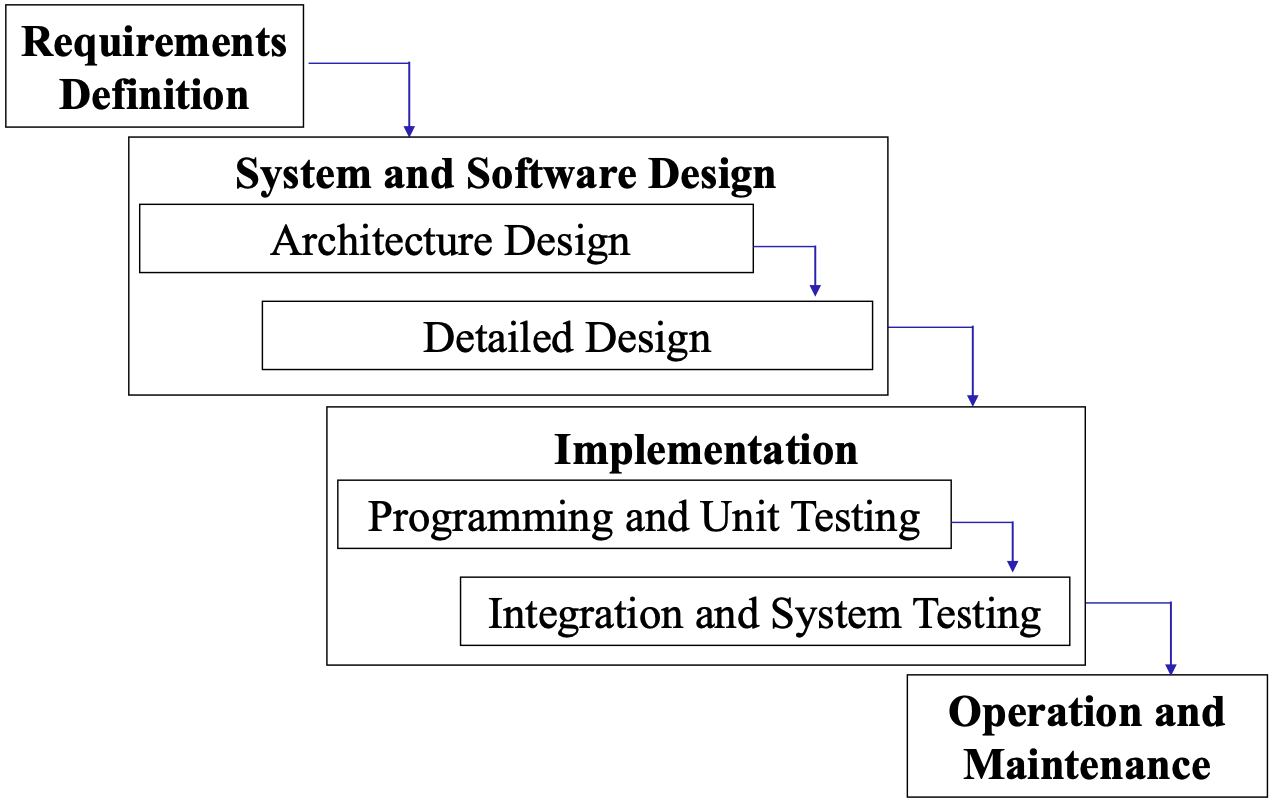
\includegraphics[width=0.5\linewidth]{imgs/1 - cascata.png}
    \label{fig:modello_cascata}
    \caption{Modello a cascata}
\end{figure}

\subsubsection{Modello a spirale}
Diverse fasi che susseguono a spirale, la gestione del rischio viene gestita
tramite prototipazione che permette di testare i prodotti.

I pro:
\begin{itemize}
    \item prevenzione dei rischi
    \item completezza della documentazione
    \item flessibilità
    \item elevata usabilità
    \item buon design
    \item facilità di manutenzione
    \item ridotto costo di sviluppo
\end{itemize}

I cons:
\begin{itemize}
    \item modello costoso
    \item riservato ad esperti e a progetti costosi
\end{itemize}

Il prototipo è un'implementazione limitata del sistema, rappresentanti solo alcuni aspetti alla volta.

\begin{figure}[h!]
    \centering
    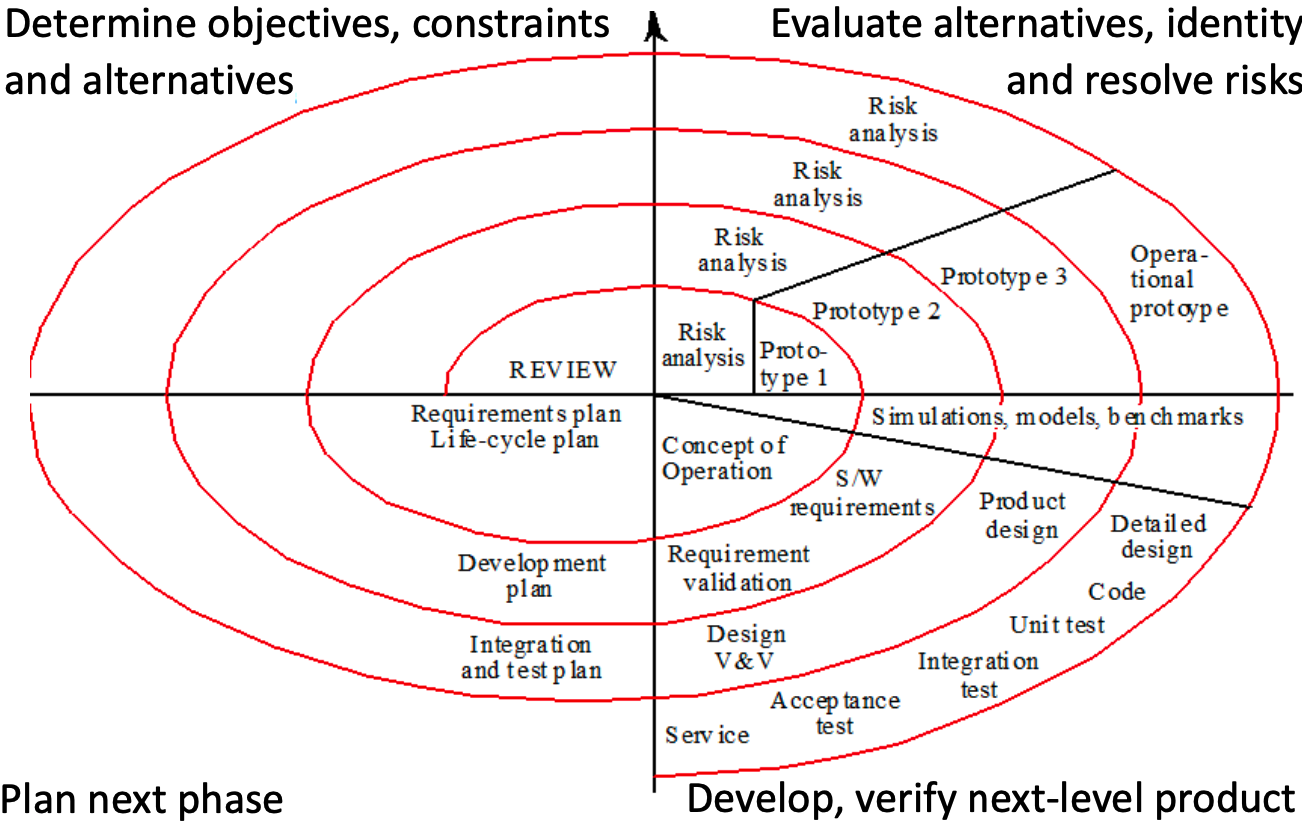
\includegraphics[width=0.5\linewidth]{imgs/2 - spirale.png}
    \label{fig:modello_spirale}
    \caption{Modello a spirale}
\end{figure}

\subsubsection{Sviluppo incrementale}
Modello che si suddivide in fasi:
\begin{enumerate}
    \item raccolta dei requisiti
    \item versione iniziale
    \item fase di design
    \item fase di implementazione
    \item produzione di versione finale
\end{enumerate}

I pro:
\begin{itemize}
    \item naturale presenza di prototipi ad ogni aggiunta di features
    \item basso rischio di fallimento
    \item qualità di testing in base alla priorità
\end{itemize}

I cons:
\begin{itemize}
    \item scarsa visibilità d'insieme
    \item sistemi mal strutturati
    \item skill speciali necessarie
\end{itemize}

Adatto a progetti piccoli o parti di progetti grandi.

\begin{figure}[h!]
    \centering
    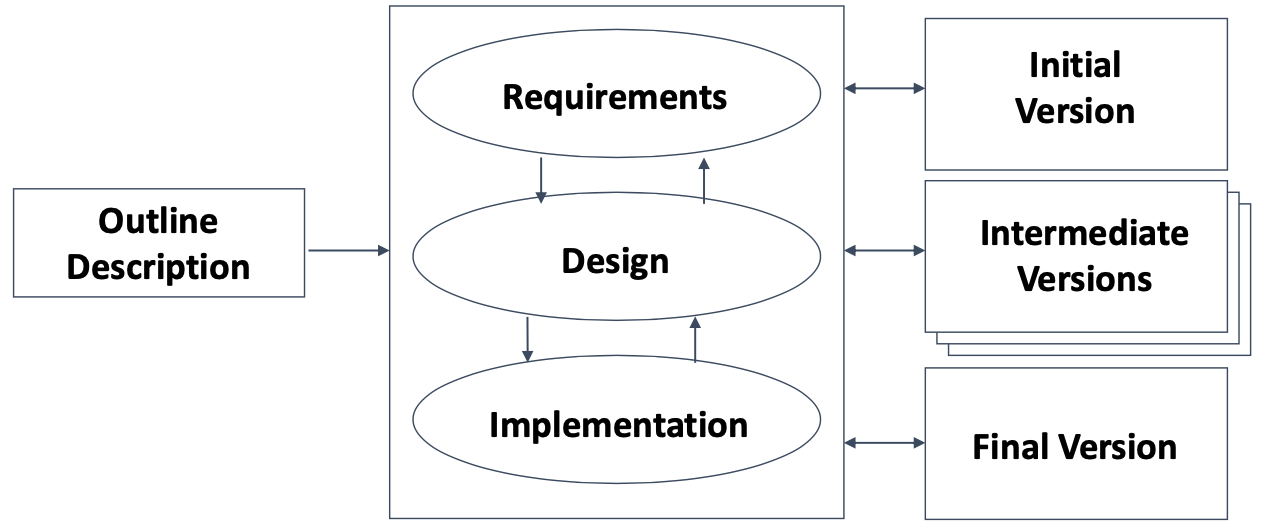
\includegraphics[width=0.5\linewidth]{imgs/3 - incrementale.png}
    \label{fig:modello_incrementale}
    \caption{Modello a incrementale}
\end{figure}

\subsubsection{Sviluppo guidato dai test}
Vengono prima scritti i test e poi l'implementazione mettendo le difficolta in primo piano.

Rende il debug più semplice.

Si aggiunte il nuovo test e poi la features cosi da veriicare che tutti i test 
precedenti siano validi.

\subsubsection{Sviluppo agile}
Questo modello di sviluppo è basato sul concetto di delivery del prodotto continuo 
avendo delle features in continua evoluzione.

Il cliente è al centro dello sviluppo, il team si autoorganizza e le features 
vengono aggiunte man mano.

Essendoci la mancanza di planning il team deve essere esperto per non perdersi.


Spesso si creano documentazioni sbagliate o incomplete.

\subsubsection{Extrem programming}
L' XP viene scelte quado i requisiti cambiano velocemente, i team sono ridotti
e affiatati(pair programming per esempio).

Tipo di programmazione agile, basato sul design semplice, release minori,
refactoring continuo, alta semplicità.

\begin{figure}[h!]
    \centering
    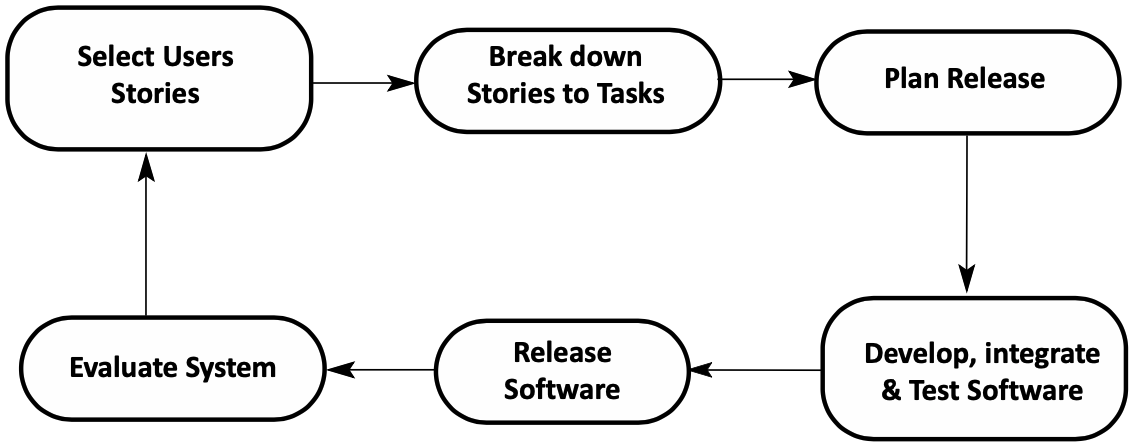
\includegraphics[width=0.5\linewidth]{imgs/4 - xp.png}
    \label{fig:modello_xp}
    \caption{Modello a extrem programming}
\end{figure}

\subsection{Software riusabile}

È comodo lavorare per \textbf{microservizi atomici}, di modo da usarli in seguito 
se si affronta un problema simile, un'esempio sono le API, è sempre meglio riusare qualcosa 
che riscriverlo da zero.

Questo "\textit{mindset}" riduce i temi e i costi di sviluppo nel luno periodo.

Il contro è il fatto che i microservizi non sono fatti espressamente per una task specifica
e si va a sacrificare qualche requisito.


\section{T2 - Coding, Debugging, Testing}
Lo stile di coding è importante perchè un programma viene scritto una volta e letto
spesso da altri!

Stare a ttenti ai layout, nomi, commenti, ecc\dots

\subsection{Legge di Ambler per gli standard}
Più uno standard è adottato e più sarà facile farlo usare al proprio team.

Non perdere tempo adietro a standard scemi.

Se hai dei dubbi usa gli standaard di google che sicuramente ne sanno più di me e te.
\textbf{\href{https://google.github.io/styleguide/}{standard di google}}


Solitamente si hanno degli standard aziendali e questi standard vanno a chiarire aspetti come:
\begin{itemize}
    \item nomenclatura
    \item formattazione
    \item formato
    \item contenuto
\end{itemize}

\subsection{Coding practices}
\begin{itemize}
    \item indentazione
    \item whitespaces
    \item naming, commenting
\end{itemize}

Fondaentale è spiegare i compiti delle classi, funzioni e procecssi complessi.

Utilizzare uno standard permette ai collechi di non dover riscrivere il codice.
Rendendo più semplice le iterazioni del codice successive.

\subsection{Gestione degli errori}
Si fa un distinguo fra il prima, durante e dopo:
\begin{itemize}
    \item prrevenzione
    \item rilevamento
    \item recupero
\end{itemize}

Per debuggare, bisogna riconoscere l'errore, isolare la fonte, identificarne la causa,
trovare un fix, applicarlo e testarlo.

\subsection{Testing}
Permette di trovare errori ma non la loro assenza, \textbf{il tester non dovrebbe
essere il programmatore}.

\subsubsection{Unit testing}
Test di singoli componenti.

\subsubsection{Integration testing}

L'intero sistema è visto come insieme di sottositemi, l'obbiettivo è quello di testare tutte le interfacce e le 
interazioni fra i sottositemi.

\subsubsection{System testing}
test dell'intero sistema per vedere se rispetta i requisiti funzionali.

\subsubsection{Functional testing}

Verifica delle funzionalità del sistema, test basati sui requisiti del progetto.

\subsubsection{Performance testing}
Test in situazioni estreme(stress testing, volume testing, recovery testing, penetration testing).

\subsubsection{Acceptance testing}
Il sistema è pronto per la produzione??

Test scelti ed effettuati dal cliente.(alpha e beta test)

\section{T3 - System Modelling and UML}

Rappresentazione astratta del sistema e dei problemi, si dedvono introdurre i componenti essenziali mediante una noazione
consistente.

Il system modelling deve essere \textbf{predictive}(prima del development), \textbf{extracted}(da un sistema 
esistente) e \textbf{prescriptive}(definire regole per l'evoluzione del software).

\subsection{UML}
UML è semplice, espressivo, utile, consistent, estensibile.

\section{T4 - Requirements engineering}

Gli scopi dell'ingegnerizzazione dei requisiti è \textbf{identificare} i servizi necessari
e i constrait, \textbf{definire} offerta e contratto, \textbf{ottenere} tutte le informazioni
necessarie al design.

Si cerca di ottenere requirements:
\begin{itemize}
    \item validi(reali necessità)
    \item non ambigui
    \item completi
    \item comprensibili
    \item consistenti
    \item prioritizzati
    \item verificabili
    \item modificabili
    \item tracciabili
\end{itemize}

\subsection{Classificazione dei requirements}
\subsubsection{Requisiti funzionali(features di sistema)}
Descrivono funzionalità di sistema o di servizio, come input di dati, output, 
operazioni svolte, workflow, autorizzazioni.

\subsubsection{Requisiti non funzionali(features di sistema)}

Descrivono i limitti di parti del sistema e del suo sviluppo.

Specificano criteri per giudicare l'operato del sistema.

\subsubsection{Requisiti del dominio(features di sistema)}
Derivato dal campo di utilizzo del software.

\subsubsection{Requisiti volatili(natura statica/dinamica)}
\begin{itemize}
    \item mutable requirements = cambiano nel tempo(tasse, nomative, ecc)
    \item emergent requirements = cambiano quando il cliente capisce di più il sistema
    \item consequential requirements = emergono con l'informatizzazione del sistema che non lo era
    \item compatibility requirements = emergono dal dover interfacciare il sistema con altri sistemi 
\end{itemize}

\subsection{Rischi}
I rischi della stesura dei requisiti possono essere:
\begin{itemize}
    \item imprecisioni
    \item conflitti tra requisiti
\end{itemize}

\subsection{Documento di specifica dei requirements}

Questo documento specifica i requisiti del sistema, includendo una definizione
e una specifica.

Prende il nome di system specification se include direttive su harware e software.

Software Requirements Specification (\textbf{SRS}) se include solo specifiche software.


Un \textbf{SRS} deve includere:
\begin{itemize}
    \item introduzione
    \item descrizione generale
    \item features
    \item requirements
\end{itemize}

Il linguaggio naturale usato per stilare questo documento implica ambiguità,
per questo si ricorre a una struttura ben definita per evitare ambiguità.

\section{T5 - Requirements ecgineering and UML}
\subsection{Use case diagram}
In questo diagramm vengono inclusi tutti i casi di utilizzo del sistema,
da parte dei vari attori che rappresentano gli utenti.

Il \textbf{System boundary} divide l'interno dall'esterno del sistema.

\subsection{Class diagram}

Diagramma che rappresenta le classi tramite:
\begin{itemize}
    \item gli attributi(pubblici con +, privati con - e \# per i protetti)
    \item le funzioni delle classi
\end{itemize}

\subsubsection{Associazione}
Quando una classe svolge il ruole di variabile all'interno di un'altra classe,
questa connessione deve essere rappresentata, si usano:
\begin{itemize}
    \item cardinalità
    \item direzione
    \item constraint
    \item ruoli
\end{itemize}

\begin{figure}[h!]
    \centering
    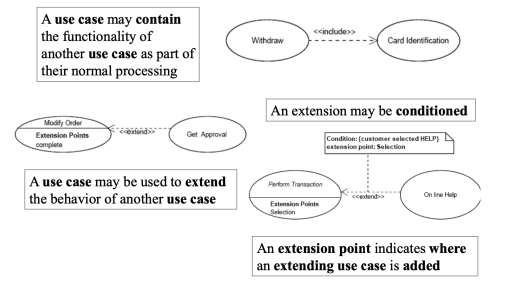
\includegraphics[width=0.5\linewidth]{imgs/5 - associazione.png}
    \label{fig:associazione}
    \caption{Associazioni}
\end{figure}

\pagebreak
\subsubsection{Gneralizzazione e nesting}

La generalizzazione indica \textbf{eretidarietà}, nesting indica che una classe 
è nestata nella classe dove arriva l'operatore.

\begin{figure}[h!]
    \centering
    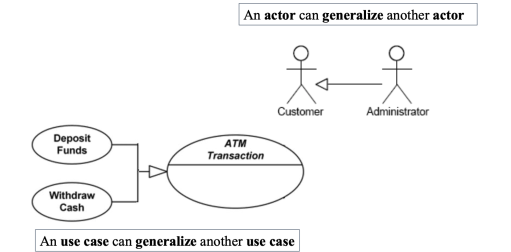
\includegraphics[width=0.5\linewidth]{imgs/6 - generalizzazione e nesting.png}
    \label{fig:generalizzazione_nest}
    \caption{generalizzazione e nesting}
\end{figure}

\subsubsection{Dipendenza e realizzazione}
\begin{itemize}
    \item \textbf{dipendenza} = relazione debole tra client e supplier
    \item \textbf{realizzazione} = relazione tra specifica e implementazione
\end{itemize}

\subsubsection{Aggregazione e composizione}

L'aggregazione rappresenta un elemento composto da altri elementi minori.


\begin{figure}[h!]
    \centering
    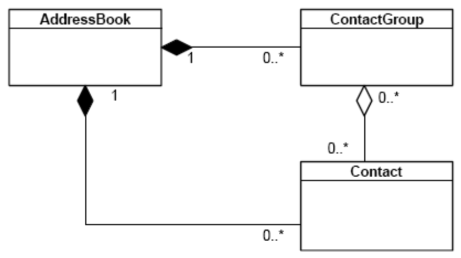
\includegraphics[width=0.3\linewidth]{imgs/7 - aggregazione.png}
    \label{fig:aggregazione}
    \caption{Aggregazione e composizione}
\end{figure}

\subsection{Sequence diagram}
Usa un timeline verticale per rappresentare l'interazione tra le classi.

Ci possono essere comunicazioni sincrone e asincorne.
\subsection{Activity diagram}
Diagramma che rappresenta un'operazione eseguita nel sistemasa con rappresentazione
dell risorse utilizzate(io, disk, banda, ecc)

\subsection{Robustnes diagram}

Diagramma UML semplificato che appresena gli use cases verificandone la corretteza, 
completezza e requisiti.

\section{T6 - Feasability and requirements elicitation}
Per ottenere le informazioni necessarie dobbiamo identificare le fonti, acquisire i dati,
verificarli e sintetizzarli.

Le varie persone interessate al progetto possono essere suddivise cosi:
\begin{itemize}
    \item stakeholder: interessato nel progetto
    \item developer: produce con pochi errori
    \item project managment: budget, scadenze
    \item investor: velocizzazione del progetto
    \item cliente e utente: usabilità e workflow
\end{itemize}


\subsection{Tecniche di elicitation}
(elicitation = tirare fuori le informazioni)
\subsubsection{Document analysis}

Analizzare i documenti e insieme agli stakeholder verificare la correttezza dei dati.

\subsubsection{Observation of the work environment}
Apprendere informazioni importanti osservando il lavoratore.
\subsubsection{Questionario}
Determinare i fatti e leopinioni con un questionario.
\subsubsection{Interviste}
Decidere chi intervistare e acquisire i dati.
\subsubsection{Scenari e casi di utilizzo}
Esempi IRL(In Real Life) di come il sistema verrà usato.

\subsection{Attività di supporto all'elicitation}
\subsubsection{Brainstorming}
composto dalle fasi storm(spara idee) e calm(analizza idee)
\subsubsection{Focus group}
simile al brainstorming
\subsubsection{Prototipi}
Esecuzone di una task e si analizza lasituazione facendo emergere problemi
e soluzioni.

\section{T7 - Use cases}

Gli use cases sono scenari plausibili che sfruttano i diagrammi UML.

Ogni requirements deve essere mappato da almeno un use case.


\subsection{Componenti principali}
Lo use case deve definire lo stato precedente del sistema,
l'ordine degli eventi, le alternative, situazioni eccezionali e i risulati.
Deve menzionare gli attori che prendono parte al sistema, i problemi di design,
i diagrammi di relazione. 

Ecco delel guidelines:
\begin{itemize}
    \item non pensare all'implementazione
    \item essere pessimistici
    \item elencae gli scenari funzionanti
    \item elencare tutti i possibili use cases
    \item utilizzare un formaato standard
    \item utilizzare verbi appropriati
    \item documentare bene le situazioni eccezionali
    \item non rappresentare singoli step come use cases
\end{itemize}



\begin{figure}[h!]
    \centering
    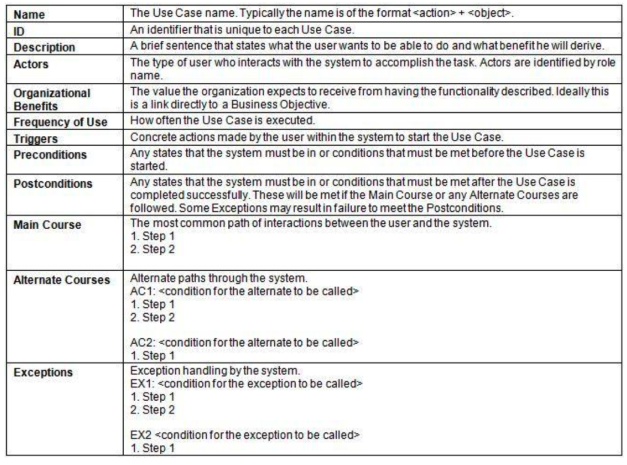
\includegraphics[width=0.6\linewidth]{imgs/8 - use case template.png}
    \label{fig:use_case}
    \caption{Tamplate per i casi di utilizzo}
\end{figure}

\section{T8 - Requirements}
L'analisi dei requisiti permette di raffinare e strutturare i requisiti in 
modo da renderli più chiari, precisi e formali.


\subsection{Analysis classes}
Il concetto è quello di astrarre le entità del problema.

\subsection{Classes discovering techniques}
\subsubsection{Noun verb analysis}
Analisi che sfrutta i contenuti delle specifiche del progetto.
Necessita di completezza del documento molto alta.

\subsubsection{Use case driven approch}
Approccio che sfrutta fli scenari degli use cases.
\subsubsection{Common class patterns}
Analisi basata sulla teoria della classificazione generica degli oggetti.

Fornisce linee guida, ma non un processo sistematico per ottenere le classi.


Introduce errori di mal'interpretazioni.

\subsubsection{CRC cards}
Sono usate in specifiche sessioni di brainstorming, generalmente si 
parte dagli use cases e s icreano delle card con:
\begin{itemize}
    \item class name
    \item responsabilities
    \item collaborators
\end{itemize}

Non è un metodo sistematico, si usano le CRC cards come validazione.

Gli achievement di questo metodo sono:
\begin{itemize}
    \item Verifica la corretteza dello use case
    \item verifica la correttezza delle associazioni
    \item verifica la corretteza delle generalizzazioni
    \item trovare le classi omesse
    \item scovare opportunità di refactoring
\end{itemize}

\subsubsection{Mixed approch}
Migliore:
\begin{enumerate}
    \item Le classi iniziali provengono dalla conoscenza del dominio
    \item si sfrutta come guida il common class pattern
    \item per aggiungere altre classi si usa la noun verb analysis
    \item per verificare il lavoro si usano gli use cases
    \item per il brainstorming si usano le CRC cards
\end{enumerate}


\section{T9 - Requirement validation and managment}
\subsection{Valdation}
La validazione consiste nella verifica della correttezza dei requisiti, con obbiettivi
la completezza e i costi.
\begin{itemize}
    \item consistenza
    \item realismo
    \item verificabilità
\end{itemize}
\subsection{Requirements managment}
Si verificano gli errori, conflitti e inconsitenze.

Soddisfare il cliente e mantenere i costi bassi:
\begin{itemize}
    \item identificazione dei requisiti
    \item processo di modifica
    \item policy di tracciabilità
    \item supporto del case tool
\end{itemize}
\subsubsection{Case tool support}
non ho voglia di spiegarlo.
\subsubsection{Stati dei requirement}
tutto questo ambaradam è molto simil ad un issue tracker come git.
\begin{itemize}
    \item proposal
    \item approved
    \item rejected
    \item implementation
    \item verified
    \item deleted
\end{itemize}

Si fanno sostanzialemnte dei test con un version control e si fa il roll back
in caso di problemi.

\subsubsection{Tracciabilità}
Anche questo discorso viene gestito bene da un software tipo git.

\subsubsection{Traciability planning}
Elemeti fondamentali del planning:
\begin{itemize}
    \item tipi di stakeholder
    \item informazioni richieste
    \item dove e da chi raccogniere info
    \item dove e come mantenere le info
    \item dove e come cercare le info
\end{itemize}

Ci sono delle limitazioni per il plannign:
\begin{itemize}
    \item numero di requirements
    \item lifetime stimato
    \item livello di maturità dell'azienda
    \item dimensione progetto
    \item altri vincoli dell'utente
\end{itemize}
\setcounter{section}{11}
\section{T12 - Object constraint lenguage}
Fa parte delle specifiche UML, e segue uno standard di IBM, è un linguaggio 
formale usato per descrivere i modelli Object oriented.
\subsection{Model type}
sono classi, subclasses, classi di associazione, interfacce ed enumerazioni.

Hanno proprietà e attributi.
\subsection{Operazioni, espressioni, constraint}
I constraint sono dei valori booleani che veificano una condizioni, servono
a porre limitazioni sul tipo di valore che può avere una classe.

\begin{itemize}
    \item Migliorano la documentazione
    \item più precisione
    \item comunicazione senza ambiguità
\end{itemize}

Vari tipi di constraint:
\begin{itemize}
    \item invarianti(quando l'istanza è a riposo)
    \item precondizionali
    \item postcondizionali
    \item guard(vera prima e dopo)
\end{itemize}

\section{T13 - Design process}
Processo che permette di capire come implementare il sistema.

Si parte dai requirements e si tiene conto dei design general princilas.

\subsection{Linee guida}
\begin{itemize}
    \item esibire organizzazione modulare che fa uso intelligente di controllo tra componenti
    \item partizione in componenti logici
    \item descrivere sia dati che procedure
    \item arrivare ad interfacce che riducono la complessità
\end{itemize}

Un buon design deve implementare tutti i requirement espliciti del modello di analisi, e tutti quelli impliciti
desiderati dal cliente. Dev'essere leggibile e comprensibile, sia per chi scrive codice, sia per chi lo testa
e supporta. In generale, dovrebbe dare un'immagine generale del software, indicandone i dati, i domini
funzionali e behavioral dal punto di vista dell'implementazione.



\subsection{Stadi del design process}
\begin{enumerate}
    \item comprendere il problema
    \item identificare una o più soluzioni
    \item processo iterativo ed incrementale
\end{enumerate}

\subsection{Design as series of decisions}
Alcuni tradeoff possono essere:
\begin{itemize}
    \item funzionalità vs usabilità
    \item costo vs robustezza
    \item efficienza vs portabilità
    \item velocità di sviluppo vs funzionalità
    \item costo vs riutilizzabilità
\end{itemize}

Gli step per una decisione pesata sulle priorità sono:
\begin{enumerate}
    \item Elencare le alternative possibili
    \item elencare i pro e i contro di ogni alternativa(rispetto agli obiettivi e alle priorità)
    \item determinare se alcune alternative impediscono altri obiettivi
    \item scegliere l'alternativa che permette di raggiungere più obiettivi
    \item aggiustare la priorità per decisioni future
\end{enumerate}

\subsubsection{Approcci}
Approccio \textbf{top-down}: prima si fa il design ad alto livello del sistema,
poi si prendono le decisioni man mano che si sviluppa il sistema.


Approccio \textbf{botton-up}: prima si decidono le utilities di basso livello riutilizzabili,
poi il modo di integrarle insieme.


Approccio \textbf{mixed}: si usa top-down per scegliere la struttura ed 
il bottom-up per i componenti riutilizzabili.

\subsubsection{Attività, rischi e obiettivi}

La fase di design ha tre fasi:
\begin{itemize}
    \item design dell'architettura
    \item user interface
    \item class design
\end{itemize}

Un buon design è \textbf{flessibile, dettagliato, ben documentato e buona possibilità di managment}.

\section{T14 - Design concepts}

Un sistema sftware ha diversi possibili problemi:
\begin{itemize}
    \item rigidità
    \item fragilità
    \item immobilità(difficle riusare i componenti)
    \item viscosità(più semplice l'hack del mantenimento del design originale)
\end{itemize}


\subsection{Software design concepts}
\subsubsection{Abstraction}
L'astrazione permette di focalizzarsi su parti importanti del software senza perdersi nell'implementazione.

Permette la descrizione di un sistema come struttura a
livelli.

\subsubsection{Refinement}
processo top-down iterabile che ad ogni passo trasforma istruzioni generiche in istruzioni più specifiche.
\subsubsection{Nascondere le informazioni}


L'information hiding è strettamente legato a:
\begin{itemize}
    \item astrazione
    \item coupling
    \item coesione
\end{itemize}

\subsubsection{Modularità}

Un metodo di design può essere detto modulare solo se supporta:
\begin{itemize}
    \item decomposability(ridurre in modulli più piccoli)
    \item composability(accorpare in un unico modulo)
    \item understandability(un modulo è comprensibile senza sapere gli altri)
    \item continuity(la modifica in un modulo modifica solo lui)
    \item protection(bug in un modulo?? affligge solo qul modulo!)
\end{itemize}

I principi per il design modulare sono: linguistic modular units (i moduli devono corrispondere alle
unità del linguaggio, come pacchetti o moduli), poche interfacce, poco scambio di informazioni tra
moduli, interfacce esplicite (se due moduli comunicano, dev'essere ovvio), information hiding(tutte
le informazioni di un modulo dovrebbero essere private, se non specificatamente dichiarato il contrario, e
per l'accesso bisogna utilizzare interfacce).


\subsubsection{Coesione}
La coesione misura la chiusura di una relazione tra elementi di un componente/classe. Una coesione forte
è desiderabile perché semplifica le correzioni, le modifiche, le estensioni, riduce il testing e promuove il
riutilizzo. Abbiamo più livelli di coesione (dal più basso al più alto):
\begin{itemize}
    \item coincidental(elementi senza relazioni ma uniti per convenienza)
    \item logical(elementi che fanno cose simili)
    \item temporal(elementi attivi nello stesso tempo)
    \item procedural(elementi che compongono una singola sequnza di controllo)
    \item communicational(elementi con stesso input e stesso output)
    \item sequential(l'output di uno è l'input dell'altro)
    \item functional(elementi che soppriscono ad un funtiona lrequirement)
    \item object(operazioni tra oggetti)
\end{itemize}

\subsubsection{Coupling}

Misura l'interconnessione tra moduli. Quando è debole, i moduli sono fortemente indipendenti. Livelli di
coupling dal più debole al più forte:
\begin{itemize}
    \item no direct(nessuna dipendenza)
    \item data(solo dati necessari)
    \item stamp(passati una lista di argomenti ma solo alcuni vengono usati)
    \item control(si passano flags e altri paramentri)
    \item externl(legato a device o device drivers)
    \item common(uso di dati globali)
    \item content(modificadi dati dell'altro modulo)
\end{itemize}

Con coupling elevato i componenti sono difficili da comprendere autonomamente,
le modifiche causano bug in altri moduli e il riuso di moduli fa schifo.

Con coupling basso aumentano i costi di performance ma lo sviluppo ne gode.


\section{T15 - Objects oriente design principles}
\subsection{Principi dell'Object Oriented Design}
\subsubsection{SRP - Single Responsability Principle}
Una classe deve avere una sola ragione di cambiare.

Le modifiche ai requirements si mappano sulle responsabilità.

Avere tante classi con responsabilità separate semplifica e rende il design flessibile.

\begin{quotation}
    \textit{
        In programming, the Single Responsibility Principle states that every module or class should have
responsibility over a single part of the functionality provided by the software.
    }
\end{quotation}


\subsubsection{OCP - Open Closed Principle}
Un modulo deve essere aperto verso l'esterno ma chiuso all modifica.

Meglio implementare cose in classi derivate piuttosto che modificae una classe.

\begin{quotation}
    \textit{
        In programming, the open/closed principle states that software entities (classes, modules, functions, etc.)
should be open for extensions, but closed for modification. If you have a general understanding of OOP,
you probably already know about polymorphism. We can make sure that our code is compliant with the
open/closed principle by utilizing inheritance and/or implementing interfaces that enable classes to
polymorphically substitute for each other.
    }
\end{quotation}


\subsubsection{Liskov Substituotion Principle}
Le classi derivate devono adempiere alle funzioni ereditate dalle classi padre
altrimenti se si usa una classe derivata al posto delal padre si generano errori.

\begin{quotation}
    \textit{
        More generally it states that objects in a program should be replaceable with instances of their subtypes
without altering the correctness of that program.
    }
\end{quotation}
\subsubsection{ISP - Interface Segregation Principles}
Avere tante interfacce client-specific è meglio di una generica.

\begin{quotation}
    \textit{
        In programming, the interface segregation principle states that no client should be forced to depend on
methods it does not use. Put more simply: Do not add additional functionality to an existing interface by
adding new methods. Instead, create a new interface and let your class implement multiple interfaces if
needed.
    }
\end{quotation}

\subsubsection{DIP - Dependency Inversion Principles}
I moduli di alto livello non dovrebbero dipendere da quelli di basso livello
ma dovrebbero dipendere da astrazioni.

\subsection{Principi di package cohesion}
\subsubsection{REP - Release/reuse Equivalency Principle}
Per riusare un componente non si fa copia incolla(perchè si perdono le modifiche alla libbreria) ma 
si inserisce il codice mediante una release della libreria e poi si modifica un'istanza.

\subsubsection{CCP - Common Closure Princple}
Le classi che cambiano insieme devono rimanere insieme.

\subsubsection{CRP - Common Reuse Principle}
Le classi che non sono reutilizzabili insieme non dovrebbero essere pacchettizate insieme.

\subsection{Package Coupling Principle}
\subsubsection{ADP - Acyclic Dependencies Principle}
No cicli nel grafico delle dipendenze.

\subsubsection{SDP - Stabel Dependencies Principle}
Ogni volta che un pacchetto cambia, tutti quelli che dipendono da lui devono 
essere validati.

\begin{quotation}
    \textit{
        Ovviamente tu preferisci i pacchetti stabili
    }
\end{quotation}

\subsubsection{SAP - Stable Abstraction Principle}
Il pacchetto perfetto è tanto stabile quanto astratto.

I pacchetti astratti dovrebbero essere responsabili e indipendenti, mentre 
quelli concreti dovrebbero essere irresponsabili e dipendenti.

\subsection{Attività per un buon design}
\begin{itemize}
    \item Dividi e conquista(scompore tutto in processi semplici da fare uno alla volta)
    \item Aumenta la coesione(Un sistema con alta coesione tiene insieme quello che deve stare insieme e lascio fuori il resto)
    \item Ridurre il coupling(meno interdipendenze tra moduli)
    \item Aumenta l'astrazione(meglio nascondere i dettagli e ridurre la complessità)
    \item Aumentare la riusabilità
    \item Riutilizzare design e codice esistente
    \item Programmare con l'idea di flessibilità(modifiche future)
    \item Anticipare l'obsolescenza(pensare alle tecnologie e pianificare la gestione del sistema)
    \item pensare alla portabilità
    \item pensare alla testabilità
    \item sviluppare con l'idea di difendere il software dal'utente.
\end{itemize}

\section{T16 - Design Patterns}

Un design pattern è una soluzione ricorrente ad un problema comune, che può essere usata
in modi diversi. È dipendente da linguaggio ed implementazione. I design patterns hanno vari obiettivi:
\begin{itemize}
    \item Codificare un buon design
    \item dare nomi espliciti alle strutture
    \item catturare e preservare le info sul design
    \item facilitare il refactoring
\end{itemize}

Due forme possibili: \textbf{Alexandrian} e \textbf{GoF}
\subsection{Creational patterns}
Creazione flessibile di oggetti(rendendo il sistema indipendente dagli oggetti creati).

\subsubsection{Factory method}
\textbf{Scopo}: il metodo factory fornisce un'interfaccia per creare oggetti
in una subclass, pemettendo di modificare gli oggetti creati.

\textbf{Problema}: Immaginiamo di dover creare un'applicazione che gestisca un servizio di logistica. La prima
versione utilizza solo trasporto su ruota, quindi la maggior parte del codice sta nella classe Truck. Dopo
un pò, l'app diventa popolare. Decidi di implementare anche il trasporto via mare. Aggiungere la classe
Ship richiederebbe modifiche in tutto il codice. Aggiungerne altre, pure.


\textbf{Soluzione}: Il metodo factory permette di sostituire la creazione di nuovi 
oggetti (con \textbf{new}) con chiamate a un metodo factory.

Gli oggetti geenrati così sono dei \textbf{prodotti}.

Però i prodotti devono avere l'interfaccia in comune.

\subsubsection{Abstract factory}
\textit{Capito fin li}

\textbf{Scopo}: L'abstract factory permette di creare famiglie di oggetti related senza specificare
le classi concrete.

\textbf{Problemo}: Immaginiamo di voler creare un simulatore di negozio di arredamenti. Il codice consiste di
classi rappresentanti 1) una famiglia di prodotti (sedia, divano, tavolo) 2) varianti di questa famiglia. Serve
un modo di creare oggetti in modo da matcharli con altri arredamenti della stessa famiglia. Non vogliamo
inoltre modificare il codice esistente quando aggiungiamo nuovi prodotti o famiglie.

\textbf{Soluzione}: Dichiaro le interfacce di ogni prodotto, le varianti dei prodotti
sono sottoclassi.

Poi dichiaro l'abstract factory(interaccia con lista di metodi) dove ogni metodo ritorna
una lista di prodotti astratti.

Poi estendo l'abstract ai prodotti concreti.

\subsubsection{Builder}
\textbf{Scopo}: permette di costruire oggetti un pezzo alla volta.
\textbf{Problema}: Se un oggetto ha bisogno di tanti paramentri di inizializzazione avrà un costruttore giga grosso.
\textbf{Soluzione}: si esegue prima un builder "generico" per poi dare gli altri valori all'oggetto 
con passaggi successivi.

\subsubsection{Prototype}
\textbf{Scopo}: Copia gli oggetti esistenti in un'oggetto definito.
\textbf{Problema}: Immaginiamo di avere un oggetto, e volerne creare una copia esatta. Come fare? Farlo
dall'esterno non è ideale: ci perderemmo tutti i dati privati! Inoltre, per fare il duplicato dobbiamo
conoscere la classe concreta dell'oggetto.

\textbf{Soluzione}: Si delega il processo id clonazione all'oggetto effettivo così da non perdere i dati privati.
Bisogna però implementare il metodo \textit{Clone()}.

\subsubsection{Singleton}
\textbf{Scopo}: permette di assicurarsi che una classe abbia una sola istanza.
\textbf{Problema}: 
\begin{itemize}
    \item si assicura che una classe abbia una sola istanza
    \item fornisce un punto di accesso globale alla risorsa
\end{itemize}


\textbf{Soluzione}: 
\begin{itemize}
    \item rendere il costruttore di default private
    \item creare un metodo getInstance che fa da builder
\end{itemize}


\subsection{Structural patterns}
\subsubsection{Adapter}
\textbf{Scopo}: permette ad oggetti con interaccia incompatibili di comunicare.

\textbf{Problema}: Immaginiamo di star creando un'app di monitoraggio del mercato in borsa. L'app scarica i
dati in XML da un'API. Ad un certo punto, vogliamo integrare un'altra API, che però restituisce dati in
JSON. Potremmo cambiare questa libreria, ma sarebbe un casino.

\textbf{Soluzione}: Creo un'adattatore che converte le interfacce.

\subsubsection{Bridge}
\textbf{Scopo}: permette di dividere un grande numero di classi in due 
gerarchie separate.

\textbf{Problema}: Ipotizziamo di avere una classe Shape con due subclasses: Circle e Square. Vogliamo
estendere questa gerarchia per incorporare i colori, quindi inizialmente proponiamo di creare sottoclassi
RedCircle, BlueCircle, RedSquare, BlueSquare. È palese che questo approccio non sia sostenibile per il
futuro.

\textbf{Soluzione}: Semplicemente, facciamo diventare il colore una proprietà dell'oggetto Shape. In questo modo,
switchamo da ereditarietà a composizione.

\subsubsection{Adapter vs Bridge}
Entrambi sono utilizzati per nascondere dettagli implementativi. L'adapter fa lavorare insieme componenti
incompatibili, mentre il bridge permette ad astrazioni ed implementazioni di variare indipendentemente.


\subsubsection{Composite}
\textbf{Scopo}: permette di comporre oggetti in strutture ad albero e lavorare su 
queste strutture come oggetti individuali.

\textbf{Problema}: computazionalmente una merda a meno che il software non sia a sua volta strutturato ad albero.

\textbf{Soluzione}:Il composite pattern suggerisce di lavorare su prodotti e scatole attraverso un'unica interfaccia,
che dichiara un metodo per calcolare il costo totale. In un prodotto, restituirebbe il costo del prodotto. In
una scatola, restituisce la chiamata ricorsiva a tutti i contenuti. \textit{Avete già capito dove voglio arrivare}. In
questo modo, basta chiamare il metodo di calcolo sulla scatola grande e verrà chiamato ricorsivamente su
tutti i nodi. \textit{Spaventosamente elegante.}

\subsubsection{Decorator}
\textbf{Scopo}: Il decorator permette di agganciare nuovi comportamenti ad oggetti, inserendoli in oggetti wrapper
che contengono questi nuovi behaviors.


\textbf{Problema}: non si possono coprire tutti casi con l'ereditarietà(per lo meno se sei umano).

\textbf{Soluzione}: Diventa una task di aggregazione più che di eretidarietà.

Si crea un oggetto wrapper che contiene i metodi del taghet e li chiama, così l'oggetto
 di base si interfaccia al wrapper per tutte le casistiche(tipo notifiche di facebook, whatsapp, sms, telegram, \dots).


\subsubsection{Facede}
\textbf{Scopo}: Fornisce un'interfaccia semplice per una libreria, framework o altre cose.

\textbf{Problema}: Immaginiamo di dover far funzionare il nostro codice con un set molto grande di oggetti che
appartengono ad un sofisticato framework. Dovremmo, prima di tutto, inizializzare tutti gli oggetti, tenere
traccia delle dipendenze, eseguire metodi nell'ordine corretto, e via dicendo. Il funzionamento del software
diventerebbe quindi molto dipendente da questo framework.


\textbf{Soluzione}: la facede fornisce una semplice interfaccia al sottositema complesso.

\subsubsection{Flyweight}
\textbf{Scopo}: permette di ridurre lo spazio di memoria necessario al salvataggio di oggetti.

\textbf{Problema}: Immaginiamo di dover creare un videogioco sparatutto. Decidiamo di implementare un sistema
di particelle complesso, in modo che proiettili, missili, detriti siano gestiti da oggetti. Avremmo quindi
una struttura in cui ogni particella occupa molto spazio in memoria:

\begin{figure}[h!]
    \centering
    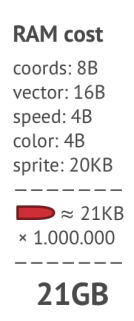
\includegraphics[height=0.2\linewidth]{imgs/9 - flyweight.png}
    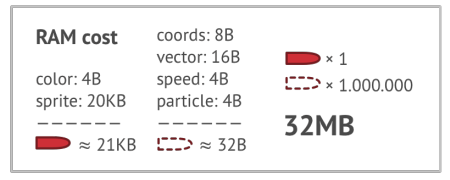
\includegraphics[width=0.4\linewidth]{imgs/10 - flyweigth 2.png}
    \label{fig:flyweight}
    \caption{flyweight}
\end{figure}


\textbf{Soluzione}: Salviamo tutte le informazioni comuni in una classe a parte.


\subsubsection{Proxy}
\textbf{Scopo}: Permette di avere un sostituto ad un oggeto, potendo eseguire operazioni prima e dopo.

\textbf{Problema}: Perché dovremmo controllare l'accesso? Per esempio, se avessimo un oggetto che usa molte
risorse di sistema ma che non utilizziamo sempre, sarebbe utile avere un lazy loading, ossia un'istanziazione
solo quando necessario.


\textbf{Soluzione}: Creiamo quindi una classe proxy che abbia la stessa interfaccia dell'oggetto desiderato. In
questo modo, agli oggetti che lo richiedono, lo passiamo al posto dell'oggetto vero e proprio. Il proxy 
crea quindi l'oggetto vero solo dopo la prima richiesta.


\subsection{Behavioral patterns}
A volte è necessario eseguire richieste agli oggetti senza conoscenze sull'operazione
 richiesta o il destinatario della stessa. Un esempio possono essere le librerie grafiche
  per bottoni e menù, che non implementano l'azione ma passano la richiesta.
   I behavioral patterns si occupano di questo: gestiscono l'assegnamento di

\subsubsection{Chain of responsabilities}
\textbf{Scopo}: permette di passare richieste attraverso una catena di handlers.

\textbf{Problema}: Immaginiamo di lavorare a un sistema di ordini online. Vogliamo restringere l'accesso al
sistema, in modo che solo gli utenti autenticati possano ordinare. Vogliamo inoltre degli amministratori,
che possano vedere tutti gli ordini. Decidiamo che questi controlli devono essere fatti in sequenza: se
l'autenticazione fallisce, non è necessario fare altre verifiche. Col tempo, si aggiungono altre verifiche: un
sanitizing dei dati, una verifica degli IP, un motore di caching. Ad ogni verifica aggiunta, il codice diventa
un porcile.

\textbf{Soluzione}: Trasformiamo quindi queste verifiche in handlers: ognuna avrà un metodo check, ed un
campo per il prossimo handler della catena.

\subsubsection{Command}
\textbf{Scopo}: trasforma una richiesta in un oggetto a se stante.


\textbf{Problema}: Immaginiamo di lavorare ad un software di text editing. Vogliamo creare una toolbar che
contenga tasti per le operazioni più importanti, con una classe Button. Cominciamo a creare subclasses
per ogni bottone necessario: OKButton, SaveButton, ApplyButton, ed ogni tasto che si aggiunge, la nostra
voglia di vivere cala. Dev'esserci un modo più furbo.

\textbf{Soluzione}: Estraiamo i dati della richiesta tramite un oggetto dall'interfaccia Command, che avrà come
implementazioni i vari tipi di comando possibili, aventi un solo metodo execute. In questo modo, 
ogni bottone chiamerà l'execute del suo Command, ma non solo: i comandi potrebbero, ad esempio, anche essere
chiamati da scorciatoie da tastiera!


\subsubsection{Interpreter}
\textbf{Scopo}: Mappa un dominio ad un linguaggio, il linguaggio ad una grammatica, e la
grammatica ad un design object-oriented gerarchico.

\textbf{Problema}: Se il dominio è
caratterizzato da un linguaggio, il problema può essere risolto tramite un interprete.

\textbf{Soluzione}: 
Modelliamo il dominio con una grammatica ricorsiva ad albero, in cui ogni regola è un nodo
o una foglia.




\subsubsection{Iterator}
\textbf{Scopo}: passa dentro ad una collection senza leekare la logica.

\textbf{Problema}: Creiamo un nostro oggetto di collection per salvare dati, con una struttura cazzutissima ed
ultra segreta, che ci permetterà di diventare milionari grazie all'intelligentissimo metodo di esplorazione dei
dati che ho. Abbiamo ora un problema: non vogliamo esporre le logiche con cui esploriamo la collection.

\textbf{Soluzione}: usiamo un iterator con i metodi get next e get prev per prendere gli oggetti.


\subsubsection{Mediator}
\textbf{Scopo}: riduce la coesione tra oggetti. 
Riduce la comunicazione 
fra gli oggetti perchè parlano attraverso lui(mediatore).



\subsubsection{memento}
\textbf{Scopo}: Permette di salvare e ripristinare lo stato degli oggetti 
senzaz rivelarne i dettagli implementativi.

\subsubsection{Observer}
\textbf{Scopo}: È un pattern che permette di definire un meccanismo di 
iscrizione per notificare 

\subsubsection{State}
\textbf{Scopo}: permette ad un oggetto di alterare il suo comportamento in base allo stato.

\subsubsection{Strategy}
\textbf{Scopo}: pattern che definisce una famiglia di algoritmi, inseriti in classi
separate e renderne gli oggetti intercambiabili.

\subsubsection{Template}
\textbf{Scopo}: permette di definire lo scheletro di un algoritmo nella sua superclasse,
poi nelle sotto classi lo si agghinda.

\subsubsection{Visitor}
\textbf{Scopo}: Separa gli algortimi dagli oggetti su cui opera.

\section{T17 - Architectural design}
Permette di comprendere l'organizzazione ed il design della struttura generale
di un sistema di software.

È il collegamento tra design e requirements engineering.

Identifica i componenti strutturali e le loro relazioni.

L'architettura è un modello di alto livello che descrive gli aspetti critici del
sistema ed è comprensibile alla maggior parte degli stakeholders, permettendo la valutazione delle proprietà
di sistema prima della sua esistenza. Fornisce strumenti e tecniche per costruire il sistema.

\subsection{Software architecture}

Software architecture sono gli aspetti rilevanti dell'architettura.

Essa è una traccia che identifica
componenti, interazioni, interconnessioni ed è definita in modo formale o informale. È fondamentale avere
un vocabolario condiviso e ricco.


\subsection{Elementi architetturali}
Un subsystem è un sistema unico, le quali operazioni sono indipendenti dai servizi di altri subsystems. Un
modulo è un componente di sistema che fornisce servizi ad altri componenti, ma non può essere considerato
un subsystem.

\subsubsection{Componenti}
Essi sono unità di computazione o data stores: clients, servers, databases, filtri, layers.
Possono essere semplici o composti(subsystem). Un architettura consistente in più componenti compositi
è un sistema di sistemi.

\subsubsection{Connettori}
Sono elementi architetturali che modellano le interazioni tra componenti e le regole che le
governano. Le interazioni si dividono in semplici (chiamate procedurali, variabili condivise) e comples-
se/semantically rich (client-server, database access, async, piped data streams)


\subsubsection{Configurazioni}
Sono grafi connessi di componenti e connettori che descrivono strutture architetturali
identificanti connettività, proprietà concorrenti/distribuite, aderenza ad euristiche/stili. I componenti
compositi sono configurazioni.



\subsection{Architectural design process}
Tre fasi:
\begin{itemize}
    \item System structuring(decompongo in sottosistemi e identifico la comunicazione fra sotto sistemi)
    \item Control modelling(scegliere un modello di controllo tra le parti)
    \item Modular decomposition(decompongo i subsystem in moduli)
\end{itemize}

\subsubsection{Box and line diagrams}
Sono diagrammi semplici ed informali che mostrano i subsystem e le loro relazioni. Mancano di semantica,
non mostrando i tipi di relazioni o le proprietà. I requisiti per la semantica dei modelli dipendono da come
il modello è usato.

\subsubsection{Software architecture views}
\begin{itemize}
    \item logical view(astrazioni chiave del sistema)
    \item process view(mostra interazioni dei processi)
    \item development view(decomposizione del software)
    \item physical view(hardware)
\end{itemize}

Gli step per questo design sono capire i requirements, definire l'architettura, rappresentare e
comunicare l'architettura, valutare l'architettura. Si utilizzano implementazione, miglioramento e
manutenzione.


\subsubsection{Non functional requirements}
\begin{itemize}
    \item performance
    \item security(architettura a strati)
    \item safety(trovare features con possibili falle di sicurezza)
    \item availability(includere componenti rindondanti)
    \item maintenability(usare componenti sostituibili e di cui si possa fare il fine-grain)
\end{itemize}


\subsubsection{Euristica dei subsystem}
Bisogna assegnare oggetti identificati nello stesso use case, allo stesso subsystem. Creare un subsystem
dedicato per oggetti atti al movimento di dati tra subsystems. Minimizzare il numero di associazioni tra
subsystem boundaries. Tutti gli oggetti nello stesso subsystem devono essere funzionalmente collegati.


\subsubsection{layering e partitioning}
Sono tecniche utili ad ottenere un basso coupling, che permettono di suddividere un sistema in subsystems.
Il layering divide il sistema in strati che forniscono servizi allo strato più alto. 
Così, uno strato dipende solo da livelli più bassi e non conosce quelli più alti. Il partitioning divide un sistema in subsystems
indipendenti.


\subsubsection{Architecture reuse}
I sistemi nello stesso dominio spesso hanno architetture simili: nascono quindi dei pattern/stili che
catturano l'essenza di un'architettura.

\subsection{Architectural patterns}
Sono descrizioni di una buona pratica di design, testata in diversi ambienti, ed includono informazioni sul
loro utilizzo. Sono rappresentati da tabelle e grafici.


\subsubsection{Model-View-Control}

Utilizziamo l'MVC quando abbiamo più modi di vedere ed interagire coi dati, e non abbiamo conoscenza
dei futuri requirements dell'interazione coi dati. I dati e le rappresentazioni possono così cambiare indipendentemente, e abbiamo più views degli stessi dati. Aumenta però la complessità del codice. Abbiamo
tre componenti:
\begin{itemize}
    \item Model(tiene e gestisce i dati)
    \item View(Presenta i dati all'utente)
    \item Control(risponde agli input e interagisce con i modelli)
\end{itemize}

\subsubsection{Layered Architecture}
Qui, ogni layer fornisce dei servizi a quello sopra. Il più basso contiene i core services. Si utilizza quando
dobbiamo creare nuove parti sopra sistemi esistenti, e lo sviluppo è basato su vari team che lavorano a
funzionalità diverse. Risolve anche i requirements di sicurezza multi-level. È un ottimo sostituto dei layer
di implementazione, supporta la ridondanza, ma ha problemi di performance e rende difficile separare
nettamente i layers.

\subsubsection{Repository}

La repository è accessibile a tutti i componenti, che non interagiscono tra loro ma solo con la repository,
che gestisce tutti i dati. Viene utilizzato quando abbiamo grandi volumi di informazioni e l’inclusione
di dati nella repo triggera un'azione. Ha componenti indipendenti, propagazione dei cambiamenti, data
management consistente, ma rischio di failure, comunicazione inefficiente e difficoltà di distribuzione della
repo.

\subsubsection{Client-Server}

Utilizziamo client-server quando i dati devono essere accessibili da più posizioni, ed il carico è variabile
(distribuzione dei server). Facilita la distribuzione di server e funzionalità, ma ogni server è un punto di
failure, abbiamo performance imprevedibili, e problemi di gestione quando i server hanno diversi proprietari.

\textbf{Thin e Fat client} Un thin client implementa l'interfaccia grafica, delegando al server ed alla rete le
operazioni più pesanti. Un fat client, invece, esegue l'applicazione localmente, ed è quindi più complesso e
potente. Gli aggiornamenti vanno installati su tutti i clients.


\subsubsection{Pipe and filter}
Il processo dei dati in un sistema è organizzato tramite una sequenza di componenti di processing, ognuno
dei quali esegue una tipologia di trasformazione dei dati, i quali scorrono da un componente all’altro.
Si utilizza in applicazioni di data processing nelle quali gli input sono processati in stadi separati per
generare output. Un esempio sono i compilatori. Si prestano bene al riutilizzo ed ai business processes.
Hanno evoluzione semplice e implementazione sequenziale/parallela. Devono però avere un formato di data
transfer condiviso, e codificare/decodificare i dati.

\subsection{Application architectures}
I sistemi di applicazioni possono essere raggruppati per il tipo di business. Siccome i business hanno molto
in comune, i loro sistemi applicativi tendono ad avere un'architettura comune che riflette i requirements.
Un'architettura generica può essere configurata e adattata per creare un sistema che ha specifici require-
ments. Le application architectures sono un punto di partenza per il design, utilizzabili come checklist,
come modalità organizzativa, come mezzo di riutilizzo, come vocabolario.


\subsubsection{Centralied vs Decentralized}
Il design centralizzato rende facili le modifiche nella control structure, penalizzando però le performance
del singolo control object. Quello decentralizzato divide le responsabilità, funziona bene con l'Object-
Oriented e permette di dividere il carico. Per scegliere, osserviamo i sequence diagrams ed i control
objects, verificandone la partecipazione. Se il sequence diagram assomiglia a una forchetta, centralizzato,
se assomiglia a una sedia, decentralizzato. C'è scritto veramente? I sequence diagrams sono derivati dagli
use case.



\subsubsection{Procedure vs event driven}
Nel procedure driven, il controllo è nel codice del programma e l'utente ha poco controllo. Nell'event driven,
il controllo risiede in un dispatcher che chiama funzioni via callbacks; l'utente ha qui molto controllo.

\subsubsection{Vantaggi di una system architecture esplicita}
\begin{itemize}
    \item Comunicazione tra stakeholder(discutere del sistema)
    \item analisi del sistema
    \item riutilizzo in larga scala
    \item definizione di strutture di divisione del lavoro
\end{itemize}

Il design dell'architettura è uno dei primi passi della metodologia agile, perché il refactor futuro è molto
costoso.


\section{T18 - User Interface Design}

Gli utenti di un sistema spesso giudicano più l'interfaccia delle funzionalità: un'interfaccia realizzata male
può causare errori o far disinstallare il software. Nel design, bisogna considerare i fattori umani: memoria
a breve termine limitata, errori, capacità differenti, preferenze di interazione diverse. Dobbiamo quindi
matchare le skills, esperienze ed aspettative degli utenti,
considerandone però anche i limiti e le possibilità
di errore. È utile basarsi su un set di design principles:

\begin{itemize}
    \item User familiarity(interfaccia user oriented)
    \item consistenza(consistenza dell'insieme)
    \item minimal surprise(un determinato comano funziona in maniera conosciuta dall'utente)
    \item recoverability(resiliente agli errori dell'utente)
    \item user guidance(sistemi di aiuto)
    \item real word mapping(layout famiglaire per le informazioni)
    \item consistency(futures simili nello stesso posto)
    \item less is more(feature meno importanti non devono essere in mezzo ai coglioni)
    \item anticipation(nascondere features inaccessibili)
    \item customization(per utenti avanzati features fighe)
    \item transparency(l'interfaccia non deve coprire altri contenuti)
    \item contiguity(testi esplicitanti vicino a icone grafiche)
    \item memory load(ricordare all'utente i dettagli)
    \item user control(identificare il responsabile delle azioni)
    \item speak user's lenguage(istruzioni comprensibili)
\end{itemize}

Alcuni tipi di componenti:
\begin{itemize}
    \item windows
    \item icons
    \item menus e pulsanti
    \item pointing
    \item graphic element
\end{itemize}

\textbf{Direct} manipulation L'utente si sente in controllo del computer, ci mette poco ad imparare, ottiene
feedback immediati. Però, la derivazione di un information space model è difficile, la navigazione può
essere complessa e quindi richiedere molte risorse.

\textbf{Menu} I comandi sono presentati in una lista, lo sforzo di scrittura è minimale, gli errori improbabili.
È possibile fornire aiuto contestuale. Però, le azioni complesse (and/or) sono difficili da rappresentare. I
menù sono adatti a poche opzioni ed utenti non esperti, perché gli esperti preferiscono i comandi testuali.

\textbf{Form} Il form permette semplice data-entry, facilità di apprendimento, possibilità di verifica. Però richiede
molto spazio a schermo e causa problemi quando l'utente non richiede esattamente ciò che è presente a
schermo.

\textbf{Command language} I comandi permettono uno sviluppo rapido, di complessità arbitraria ed interfacce
minimali. Però, gli utenti dovranno ricordare il linguaggio: non è adatto ad utenti saltuari. Faranno inoltre
errori, e sarà richiesta la possibilità di scrittura.

\textbf{Linguaggio naturale} Esso è accessibile ad utenti inesperti ed estensibile facilmente. Però, il vocabolario
è limitato e confinato a domini specifici. La tecnologia non è del tutto adatta a rendere queste interfacce
accessibili ad utenti principianti (questa slide probabilmente è stata scritta nel 2004, quando Siri e Google
Assistant non esistevano. Un aggiornamento non sarebbe male eh), ma gli utenti esperti odiano dover
scrivere molto. È necessario poter scrivere.



\subsection{Design process}

Per il design è utile sviluppare un prototipo low-fidelity, che sia semplice ed economico anche nella modifica,
in modo da far capire le caratteristiche principali senza concentrarsi sulle piccolezze estetiche. Bisogna
spiegare le convenzioni agli utenti ed è difficile mostrare i comportamenti. Il processo di design consiste in:
\begin{enumerate}
    \item analisi e comprensione delle attività dell'utente
    \item produzione di prototipi su carta e confornto con gli utenti
    \item design del prototipo dinamico e valutazione
    \item design prototipo eseguibile, valutazione e implementazione
\end{enumerate}

\subsubsection{Information presentation}
L'information presentation è costituita dallo studio di come presentare le informazioni all'utente, direttamente o trasformandole. L'MVC è una modalità che supporta più presentazioni di dati. Dobbiamo così
porci più domande:
\begin{itemize}
    \item l'utente è interessato alle info e alle loro relazioni?
    \item quanto rapidamente variano?
    \item l'utente deve poter rispondere ai cambiamenti?
    \item manipolazione diretta?
    \item testo o numeri?
\end{itemize}

Sfruttiamo i colori per supportare le
attività dell'utente in maniera intelligente e consistente, stando attenti anche agli accostamenti.




\textbf{Messaggi di errore} Una corretta rappresentazione degli errori è fondamentale. I messaggi devono essere
educati, concisi, consistenti e costruttivi.


\subsection{Valutazione della user interface}
Dopo il lavoro di design, bisogna valutarlo vs. le specifiche di usability, seguendo parametri come learna-
bility, speed of operation, robustness, recoverability, adaptability. Utilizziamo più tecniche di valutazione:
\begin{itemize}
    \item expert review
    \item questioanri
    \item registrazioni video dell'utilizzo
    \item strumenti di raccolta delle info
    \item feedback degli utenti
    \item competitive usability testing
\end{itemize}

\section{T19 - UML Diagrams for system design}

\subsection{Component diagram}
Il component diagram mostra gli elementi concettuali del business process (in UML1 erano componenti
fisici), che forniscono o utilizzano interfacce per l'interazione con altri costrutti del sistema.




\textbf{Component} Unità logica del sistema, ha interfacce definite ed è rappresentato da un rettangolo.

\textbf{Interface} Descrive un gruppo di operazioni usate o create dai componenti. Un cerchio intero rappresenta
un'interfaccia creata, mezzo ne rappresenta una required.

\textbf{Dependencies} Le dipendenze sono indicate da frecce tratteggiate.

\textbf{Ports} Le porte sono rappresentate da quadrati sul bordo. Sono usate per supportare l’esposizione di
un'interfaccia required/created.


\subsection{Package diagram}


Il package diagram serve per rappresentare la struttura dei package, dove i package 
vengon usati in progetti di grandi dimensioni per aumentare la modularità.

Qui vengono aggiunte anche le dipendenze nel disegno delle dipendenze.

\subsection{Deployment diagram}
Il deployment diagram mostra l'architettura di esecuzione del software, quindi processori, nodi, devices,
le loro connessioni e la distribuzione dei file. Utilizziamo questi diagrammi per mostrare l’hardware e
software di esecuzione.

\section{T20 - Object Oriented Desing}
L'Object Oriented Design ha lo scopo di aggiungere dettagli alla requirements analysis e all’architecture
model, prendendo decisioni riguardanti l'implementazione.
Gli obbietivi sono:
\begin{itemize}
    \item riutilizzare le conoscenze del passato
    \item riutilizzare funzionalità disponibili
    \item svuluppare la definizione di robustezza e adattabilità
    \item nuove funzioni
    \item adattare ssitema esistente a nuovo ambiente
\end{itemize}

\textbf{4 step fondamentali}:
\begin{enumerate}
    \item identificazione di soluzioni esistenti(con l'ereditarietà sfruttiamo componenti, soluzioi e design patterns) 
    \item interface specification(descriviamo bene ogni class interface)
    \item object model restructuring(miglioriamo la comprensibilità e l'estensibilità)
    \item object model optimization(miglioriamo le Performance)
\end{enumerate}


\subsection{Refactoring}
Cambio della struttura interna senza cambiare il comportamento "visto" dall'esterno.

Migliora il design del software, velocizzandolo, rende il design più comprensibile, rende il debugging più facile, permette
di programmare più velocemente. Teniamo in conto tre principi:
\begin{itemize}
    \item non si aggiungo funzioni nel refactoring
    \item verificare l'esistenza di test ottimali prima del refactoring
    \item piccoli passi localizzati
\end{itemize}

\subsection{Tecniche di riutilizzo}
\subsubsection{Ereditarietà}
Due utilizzi:
\begin{itemize}
    \item Descrizione delle tassonomie: utilizzata durante la requirements analysis, identifica oggetti del domi-
    nio che hanno una relazione, allo scopo di rendere l'analysis model più comprensibile.
    \item itemizeSpecifica delle interfacce: usata durante l'object design, identifica le signatures degli oggetti identificati, allo scopo di aumentare il riutilizzo, la modificabilità, l'estensione.
\end{itemize}

Distinguiamo, inoltre, tra inheritance (white-box reuse), e composition (black-box reuse).

Abbiamo più ragioni per le quali può essere necessaria la
creazione di oggetti:
\begin{itemize}
    \item nuovi compenenti della GUI
    \item implementazione di algoritmi
    \item classi controller e cooridnator
\end{itemize}

\subsubsection{Delegation}
Nella delegation, due
oggetti sono coinvolti nella gestione di una richiesta del client: il receiver delega le operazioni al delegate,
assicurandosi che il client non utilizzi il delegate in modo errato.

\subsubsection{Contraction}
Il goal della contraction è rendere le operazioni della superclass invisibili, implementando
metodi nella superclasse ed overridandoli con metodi vuoti nella subclass.

\subsection{package design}
Il packaging design impacchetta il design in unità discrete che possono essere modificate, compilate,
collegate, riutilizzate.

Due principi base: minimizzare il coupling,
massimizzare la cohesion. Come fare?
\begin{enumerate}
    \item partire con un'interfaccia per ogni subsystem
    \item limitare il numero di operazioni dell'interfaccia
    \item se l'interfaccia ha troppe operazioni, riconsiderare il umero di interfacce
    \item se abbiamo poche interfacce, riconsideriamo il numero di subsystem
\end{enumerate}

\subsection{Information hiding}
Per ottenere un buon information hiding, definiamo interfacce pubbliche, applicando il ”need to know”
principle: meno dettagli una classe deve sapere, più facile è cambiarla/non rovinarla con cambiamenti.





\setcounter{section}{21}
\section{T22 - testing}


\subsection{Componenti del testing}
\subsubsection{Test plan}
Il test plan è utilizzato per dimostrare che il software è privo di falle e si comporta come richiesto dai
requirements.
\subsubsection{Test specification}

Documenta lo scopo di un test; in caso di test compositi, documenta la relazione tra le parti ed il whole
test.
Descrive le condizioni che indicano quando il test è completo. In generale, è un modo per valutare i
risultati.

\subsubsection{Test oracle}
È un set di risultati predetti per un set di test, e si usa per determinare il successo del testing.
MOlto complicato da creare.

\subsubsection{Test cases}
È un set di input al sistema. Un testing di successo è basato sulla scelta dei giusti test cases.

\subsubsection{Test suite}
Ovviamente bisogna testare il codice per farlo funzionare la prima volta, facendo ad hoc testing o costruendo
una test suite.

Distinguiamo tra due tecniche di testing: glass box testing,
in cui esaminiamo il codice, e black box testing, basato sulla conoscenza del risultato atteso.


\subsection{Tipologia di testing}


\begin{figure}[h!]
    \centering
    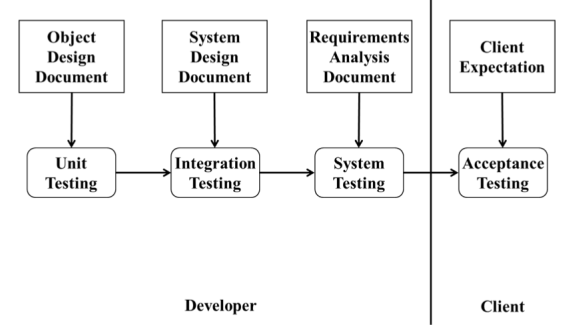
\includegraphics[width=0.5\linewidth]{imgs/11 - tipologie di testing.png}
    \label{fig:testing}
    \caption{Tipologie di testing}
\end{figure}

\subsubsection{Unit testign}
Lo unit testing testa le singole unità che compongono il sistema, allo scopo di trovare falle in algoritmi,
dati, sintassi.

Distinguiamo,
anzitutto, tra static testing(analisi, code review) e dynamic testing (black-box, white-box).


\subsubsection{Integration testing}

L'integration testing testa un gruppo di subsystems, ed eventualmente l’intero sistema. È fatto dagli
sviluppatori per testare le interfacce tra subsystems. L'intero sistema è visto come una collezione di
subsystems, determinati durante il system e object design.


\textbf{Driver} È un componente che chiama l'unità testata e controlla i test cases
\textbf{Stub/Double} è un componente che simula la presenza di un altro, rispondendo alle chiamate con dati
falsi. Non deve comportarsi esattamente come chi sostituisce, ma deve fornire circa la stessa API. Ne
distinguiamo 4 tipi:
\begin{itemize}
    \item dummy
    \item stub(forza il sistema verso il path che vogliamo provare)
    \item mock(valori hardcoded)
    \item fake(implemetazioni alternativa)
\end{itemize}

\subsubsection{System testing}
Il system testing testa l'intero sistema, ed è fatto dagli sviluppatori allo scopo di determinare se il sistema
rispetta i requirements funzionali e di performance.


I test cases sono centrati attorno ai requirements e alle funzioni
chiave, ed il sistema è trattato come una black box. Gli unit test cases sono riutilizzati, ed i nuovi test
cases vanno sviluppati.




\textbf{Performance testing} Il goal è tentare di violare i non-functional requirements, testando come il sistema
si comporta quando è sovraccaricato.


\textbf{Acceptance Testing} Il goal è dimostrare che il sistema è pronto per l'utilizzo, con test e svolti scelti
dal cliente. Distinguiamo tra alpha test, in cui si testa nell'ambiente di sviluppo, e beta test, in cui si
testa nell'ambiente del cliente.


\subsection{Object oriented tesiting}

\textbf{Object Class Testing} Un test completo di una classe testa tutte le operazioni associate, gli attributi,
tutti gli stati. L'ereditarietà rende questo test più complesso.


\textbf{Ereditarietà, polimorfismo, dynamic binding}
\begin{itemize}
    \item Ereditarietà: i metodi ereditati devono essere ritestati nelle subclasses: il contesto delle superclasses
    potrebbe essere incompleto
    \item Polimorfismo: i parametri devono avere più di un set di valori e un'operazione deve essere implemen-
    tata da più di un metodo
    \item Dynamic binding: i metodi che implementano un'operazione sono sconosciuti fino al runtime
\end{itemize}
\textbf{Continuous testing} Il continuous testing consiste in build e relativo testing ogni giorno, in modo che
il sistema sia sempre eseguibile.









\end{document}
% materia spiegata malissimo per dare un esame nel pomeriggio.